\documentclass[12pt]{report}
\usepackage[square,sort,comma,numbers]{natbib}

\bibliographystyle{abbrvnat}
\setcitestyle{authoryear,open={(},close={)}}
\usepackage[utf8]{inputenc}
\usepackage{epsfig}
\usepackage{latexsym}
\usepackage[hidelinks]{hyperref}
\usepackage{graphicx}
\usepackage[center]{caption}
\usepackage{titlesec}
\usepackage{pdfpages}


\titleformat{\chapter}[display]{\bfseries\centering}{\huge Chapter \thechapter}{1em}{\Huge}
%Load the package
%\usepackage[
%nonumberlist, %do not show page numbers
%acronym,      %generate acronym listing   -> Not used in this example (see line with %%% )
%toc,          %show listings as entries in table of contents
%section,%use section level for toc entries
%nopostdot]     %sont show . at the end
%{glossaries}
%\loadglsentries{glossary}
%Activate glossary commands
%\makeglossaries
\usepackage[nottoc]{tocbibind}


\usepackage[page,toc,titletoc,title]{appendix}
%\usepackage{refcheck}
\usepackage{datetime}

\newdateformat{monthyeardate}{%
    \monthname[\THEMONTH], \THEYEAR}

\DeclareGraphicsExtensions{.pdf,.png,.jpg}
\captionsetup{justification=centering,margin=2cm}

\begin{document}


    \title{Develop New Transformer Architecture For \\ Question and Answering(QandA)}

    \author{Nirbhay P. Tandon}

    \date{\vfill \monthyeardate\today}
        \maketitle


    \newpage
    \newpage
    \tableofcontents
    \newpage
    \listoffigures
    \listoftables
    \newpage
%\printglossary[type=\acronymtype, title=List Of Acronyms]

    \chapter{\centering Introduction}\label{c1}
        \section{Background Of The Study}\label{11}
        \section{Aims And Objectives}\label{12}
        \section{Scope Of The Study}\label{13}
        \section{Significance Of The Study}\label{14}
        \section{Structure Of The Study}\label{15}
    \chapter{\centering Literature Review}\label{c2}

    We have divided this section into 3 key subsections. Section \ref{21} deals with the early days of Question-Answering based systems using \acrshort{rnns} and the common challenges that were faced for them. We then move on to section \ref{22}, where we see the use of \acrshort{lstms}
        \section{Question Answering Using Neural Nets}\label{21}
        \section{Question Answering Using LSTMs}\label{22}
        \begin{enumerate}
            \item \citep{haighextractive};ouaguwe;ughqawoug;akuhgdfk
        \end{enumerate}
        \section{Question Answering Using Transformers}\label{23}
        Outlined below are some of the most important pieces of research that relate directly to the work done for Transformers and Q\&A based systems.
        \begin{enumerate}

            \item Work done in the field of Long short-term and gated recurrent \citep{lstm} and \citep{recurrent} neural networks, in particular, has been established as a state of the art approach in sequence modelling, transduction problems such as language modelling and machine translation.
            In their paper Attention Is All You Need,\citep{atayl} the team set out to resolve problems in the parallelization and increased compute times of recurrent models. The inherently sequential nature of RNNs causes issues in memory constraints, leading to reduced batch sizes.\\
            \begin{figure}[h!]
                \centering
                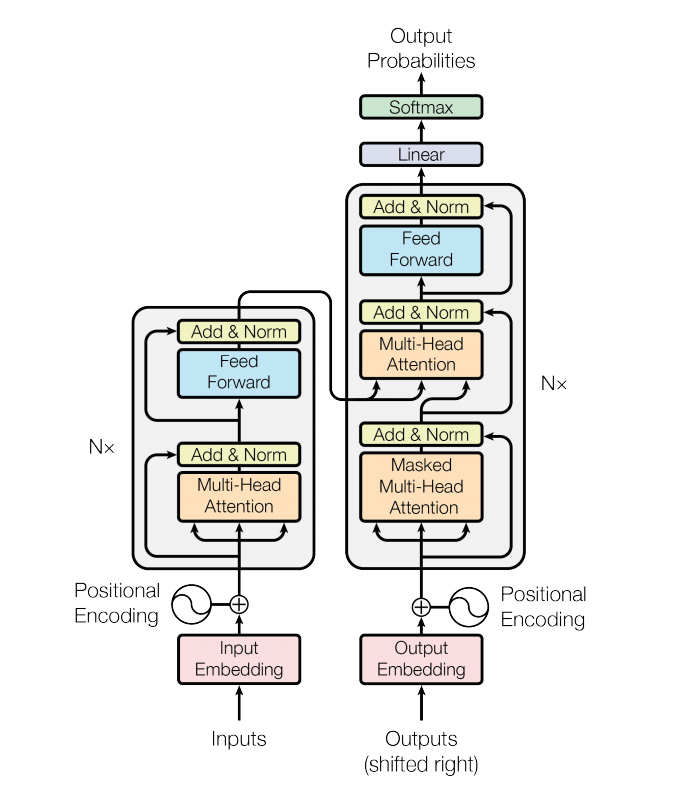
\includegraphics[scale=0.25]{transformer.png}
                \label{fig1}
                \caption{Transformer Architecture built by \citep{atayl}}
            \end{figure}
            The architecture for a \textit{Transformer} in this paper is outlined as having an encoder that maps input sequences to a continuous representation. The architecture can be seen above in Figure 1. This is then decoded into an output sequence of symbols one at a time. Each step is auto-regressive, i.e. it consumes the previously generated symbols as additional input when creating the next. This is similar to an ensemble model. Stacks of 6 encoder layers and 6 decoder layers is used.\\
            The encoder layers each have 2 sub-layers of a multi-head self-attention and the other a simple, position-wise fully connected feed-forward network layer.\\
            The decoder layer is similar to the encoder layer and has an additional 3rd sub-layer that performs multi-head attention over the output of the encoders. There is also normalization and  the outputs are prevented from attending to subsequent positions. \\ The attention mechanism can be described as mapping a query to a set of key-value pairs. This can be seen from Figure 2, below. \\The evaluations performed on the Wall Street Journal dataset\citep{wsj}, using 40k sentences, showed that even without task-specific tuning the model had better results with a fraction of the training cost.
            \begin{figure}[h!]
                \centering
                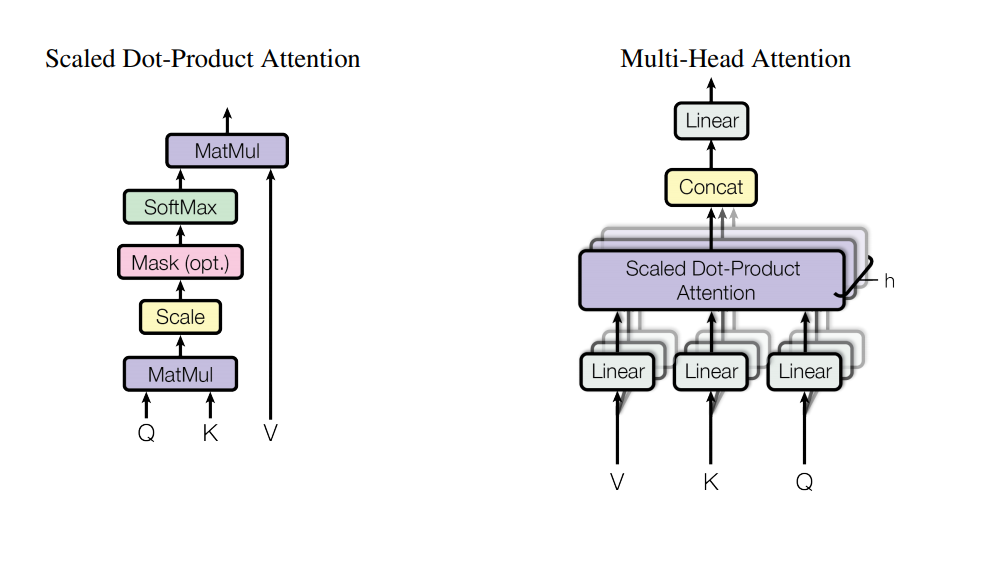
\includegraphics[scale=0.4]{multihead.png}
                \label{fig2}
                \caption{Scale Dot and Multihead Attention Models \cite{atayl}}
            \end{figure}
            \item The paper on BERT, which is \textit{Bidirectional Encoder Representations from Transformers} \citep{bert}, introduces a new language model. This model is truly fascinating in many ways. First and foremost it is designed to pre-train deep bidirectional representations using unlabelled data. This is done by jointly conditioning context in all layers to the right and left. This pre-training allows the model to be fine-tuned simply using one additional output layer. These features make this model conceptually simple and very powerful empirically.

            BERT employs language pre-training \citep{dai} which has shown significant advantages in many applications e.g. paraphrasing, language level inference etc. These tasks aim to highlight the relationships between sentences through contextual understanding as well as by using tokenized outputs.
            \begin{figure}[h!]
                \centering
                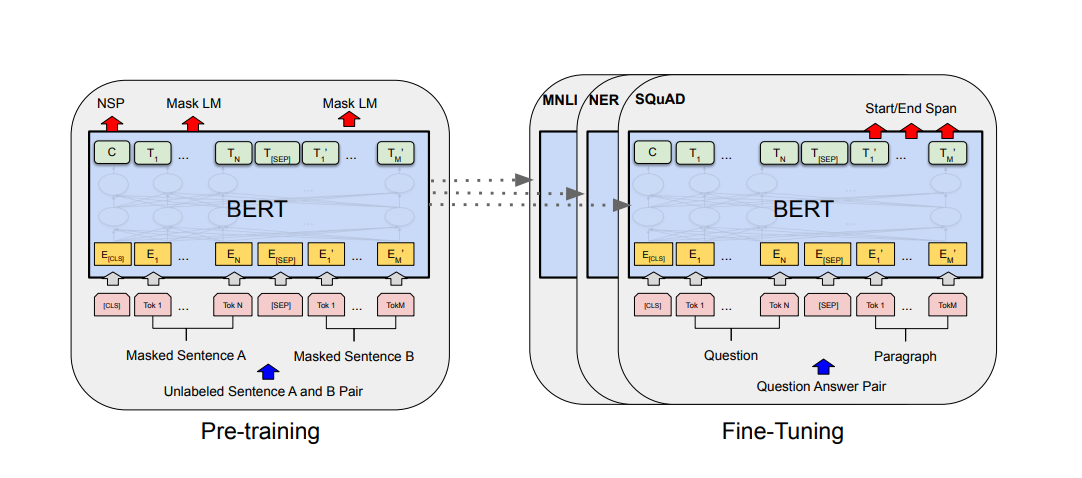
\includegraphics[scale=0.35]{BERT.png}
                \label{fig3}
                \caption{Pre-training and Fine Tuning procedures for BERT \citep{bert}}
            \end{figure}

            BERT was tested on The General Language Understanding Evaluation (GLUE) benchmark \citep{wang} which has a large number of diverse NLU tasks.
            BERT performed extremely well on the 11 NLP tasks that the authors ran it against. it showed an average accuracy improvement of 4.5\% and 7\% when compared to the previous state of the art models. Results of BERT and its significant gains make it one of the best candidate models for NLU tasks.

        \end{enumerate}

        Several advancements have been made to the BERT model to make it fast, better at understanding and even performing application-specific tasks such as Q\&A.

        The SQuAD 2.0 dataset has inspired an LSTM based FastQA \citep{fastQA} model architecture. This architecture takes cues from the work done by Hochreiter and Schmidhuber in their work on Long Short-Term Memory Architecture \citep{lstm}, to create a model specifically for end-to-end question answering systems.

        A common theme with BERT is that it takes a long time to train. Especially in the BERT based RoBERTa architecture \cite{roberta}. RoBERTa takes on average 4-5 times more time to train than BERT, however, it also shows a maximum of 20\% improvement over BERT, depending on the application. ALBERT, which is A Liter BERT, \cite{albert} was developed specifically to deal with memory limitations and reduce training times. ALBERT's XXL implementation has been documented to perform better in models trained on the BOOKCORPUS and Wikipedia ones by at least 2\% across multiple applications. In a smaller amount of time.

        However, none of these model architectures has been able to address all the problems and serve as more generic solutions to multiple end-to-end sequence encoding problems across various applications.

        Our work is primarily focused on building a fast model that allows for higher accuracy in responses specifically with Q\&A systems.

        \section{Comparison Of Techniques}\label{24}
        \section{Summary}\label{25}

    \chapter{\centering Research Methodology}\label{c3}
    \textbf{DONT DO ANY ANALYSIS HERE}
        \section{Data Selection}\label{c31}

        The SQuAD 2.0 Dataset \citep{dataset}, was developed with funding from Facebook to help address some major issues with existing datasets. Most datasets focus on questions that can be easily answered or use of automatically generated, unanswerable questions which are easily identifiable.\\
        The SQuAD 2.0 dataset resolves this by combining the SQuAD dataset along with 50,000 crowd worker generated unanswerable questions. The key feature of these being that the unanswerable questions must look similar to answerable ones. For a model to be successful on this new dataset, it must be able to answer all possibly answerable questions as well as determine when no answers are provided for a question in the given paragraph and abstain from answering. A comparative study was done for a Natural Language Understanding(NLU) task that obtained an 86\% score on SQuAD 1.1, only got 66\% on the new 2.0 dataset.
        The dataset helps bridge the gap between true NLU and machine understanding by using the concept of Relevance. Through comparisons with various datasets such as RACE, \acrshort{MCTest}, \acrshort{QASENT} etc. they have identified the missing links like negative examples, antonyms and helped fill the gap. This dataset forces the models to understand whether a paragraph span has the answer to the question posed.
        \section{Data Pre-processing And Transformation}\label{c32}
        \section{Existing Models And Benchmarks}\label{c33}
    \chapter{\centering Architecture Creation}\label{c4}
        \section{Drawbacks Of Current Architectures}\label{c41}
        \section{Proposed Architecture Improvements}\label{c42}
        \section{Architecture Refinement}\label{c43}
    \begin{appendices}
        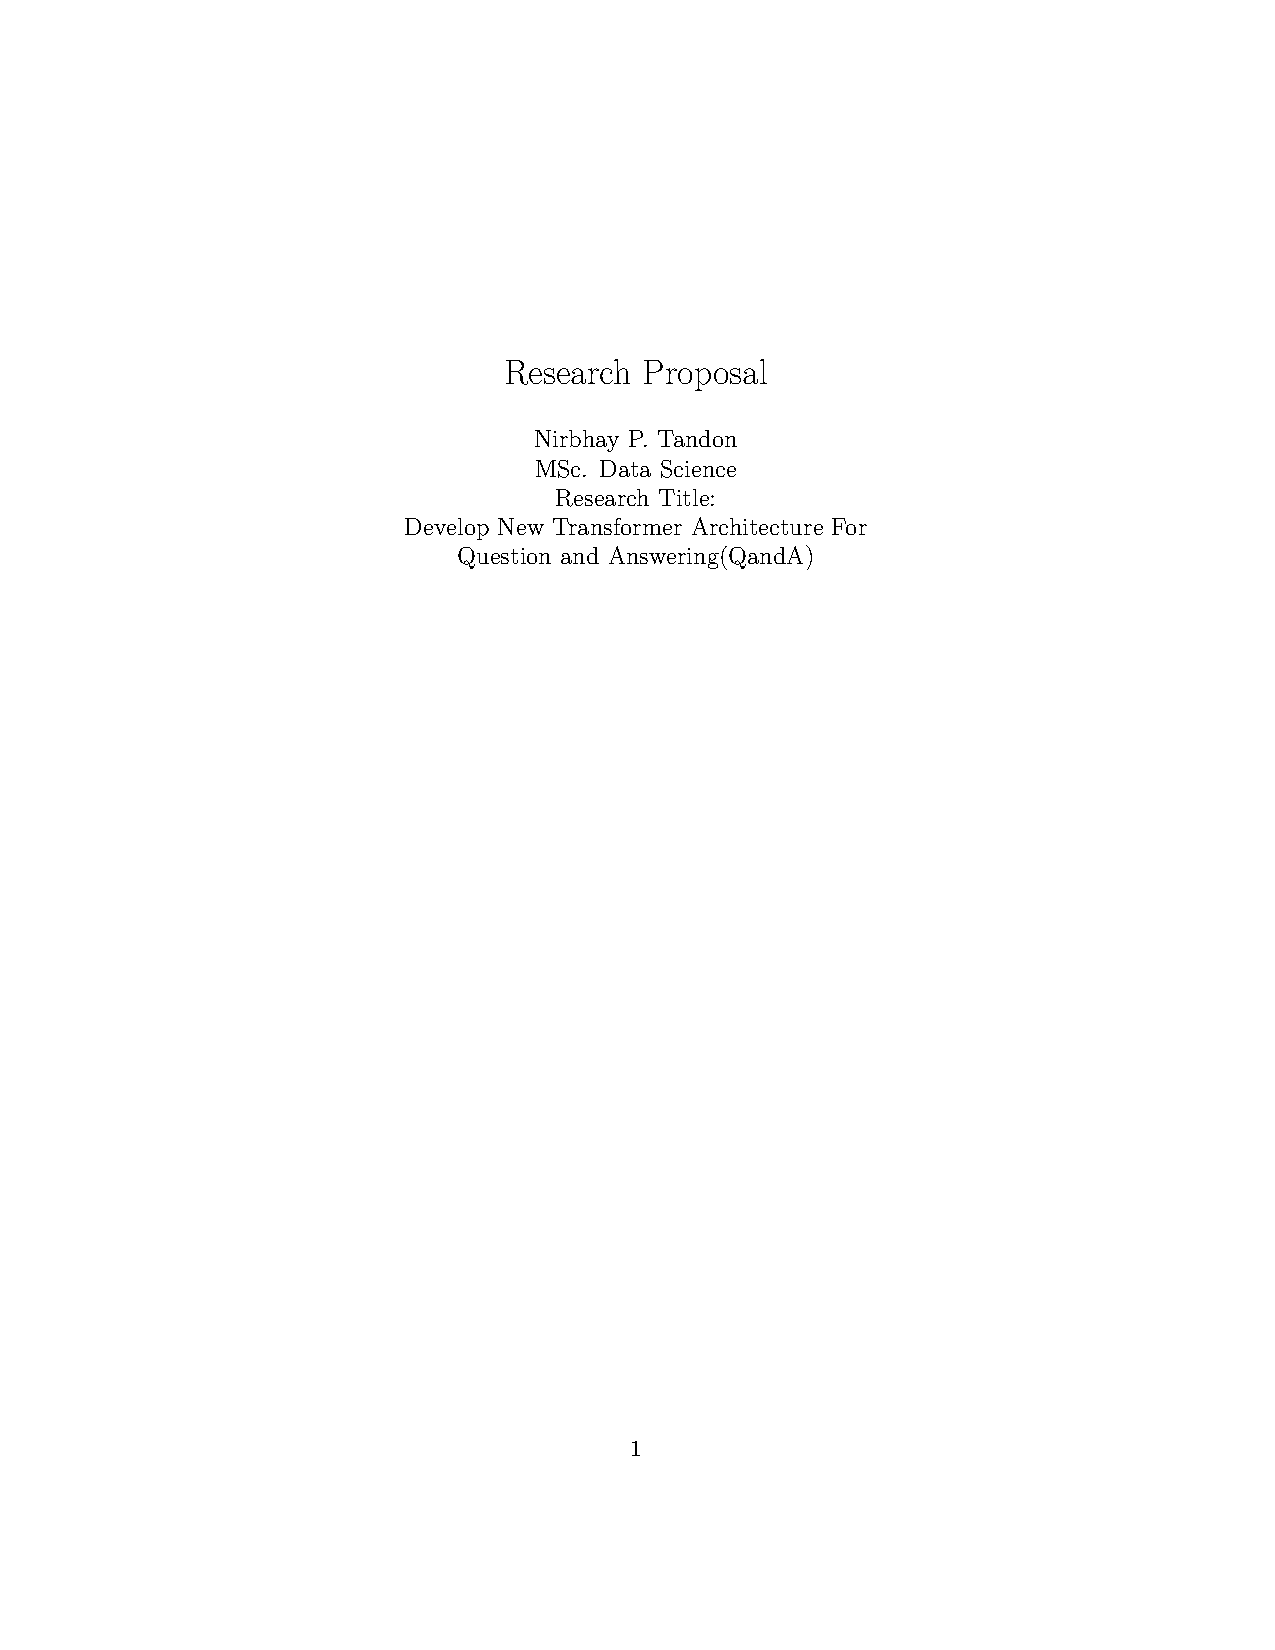
\includepdf[pages=-]{rp}

    \end{appendices}
    \bibliography{MidThesis}

\end{document}